
%\newcommand{\st}{~\text{s.t.}~}
\newcommand{\rgets}{\overset{\$}{\gets}}
%\newcommand{\ind}{\overset{c}{\approx}}
\section{NIZK Proof Systems}
We now consider a different class of Zero-Knowledge proof systems, where no
interaction is required: The Prover simply sends one message to the Verifier,
and the Verifier either accepts or rejects. Clearly for this class to be
interesting, we must have some additional structure:
both the Prover and Verifier additionally have access to a common random public string
$\sigma$ (trusted to be random by both). For example, they could derive $\sigma$
by looking at sunspot patterns. 

\section{Definitions}

\begin{definition}[NIZK Proof System]
    A \emph{NIZK proof system} for input $x$ in language $L$, with witness $\omega$, is a set of
efficient (PPT) algorithms $(K, P, V)$ such that:
\begin{enumerate}
    \item Key Generation: $\sigma \gets K(1^k)$ generates the random public string.
    \item Prover: $\pi \gets P(\sigma, x, \omega)$ produces the proof.
    \item Verifier: $V(\sigma, x, \pi)$ outputs $\{0, 1\}$ to accept/reject the proof.
\end{enumerate}
Which satisfies the completeness, soundness, and zero-knowledge properties below.
\end{definition}
Note: We will assume throughout that $x$ is of polynomially-bounded length, i.e., we are
considering the language $L \cap \{0, 1\}^{P(k)}$.


\medskip
\noindent\textbf{Completeness.} $\forall x \in L, \forall \omega \in R_L(x)$:
    $$\Pr[\sigma \gets K(1^k), \pi \gets P(\sigma, x, \omega) : V(\sigma, x,
    \pi) = 1] = 1.$$

\medskip
\noindent\textbf{Non-Adaptive Soundness.} $\forall x \not\in L$:
    $$\Pr[\sigma \gets K(1^k): \exists~\pi \st V(\sigma, x, \pi)
    = 1] = \mathsf{negl}(k).$$
The above definition is ``non-adaptive", because it does not allow a cheating
prover to decide which statement to prove after seeing the randomness $\sigma$.
We may also consider the stronger notion of ``adaptive soundness", where the
prover is allowed to decide $x$ after seeing $\sigma$:

\medskip
\noindent\textbf{Adaptive Soundness.}
    $$\Pr[\sigma \gets K(1^k): \exists~ (x, \pi) \st  x \not\in L, V(\sigma, x, \pi)
    = 1] = \mathsf{negl}(k).$$
    
\medskip
\noindent\textbf{(Non-Adaptive) Zero-Knowledge.}
    The exists a PPT simulator $S$ such that $\forall x \in L, \omega \in
    R_L(x)$, the two distributions are computationally indistinguishable:

\begin{minipage}{0.5\textwidth}
    \begin{enumerate}[itemsep=-3pt]
        \item $\sigma \gets K(1^k)$
        \item $\pi \gets P(\sigma, x, \omega)$
        \item Output $(\sigma, \pi)$
    \end{enumerate}
\end{minipage}
\begin{minipage}{0.5\textwidth}
    \begin{enumerate}
        \item $(\sigma, \pi) \gets S(1^k, x)$
        \item Output $(\sigma, \pi)$
    \end{enumerate}
\end{minipage}

\medskip
That is, the simulator is allowed to generate the distribution of randomness
$\sigma$ together with $\pi$. Note that if we did not allow $S$ to produce
$\sigma$, this definition would be trivial (a verifier could convince himself by
running the simulator, instead of interacting with $P$). Allowing $S$ to
generate $\sigma$ still keeps the definition zero-knowledge (since a verifier sees both $(\sigma,
\pi)$ together), but puts $P$ and $S$ on unequal footing.

We could also consider the adaptive counterpart, where a cheating verifier can
choose $x$ after seeing $\sigma$:

\medskip
\noindent\textbf{(Adaptive) Zero-Knowledge.}
    The exists a PPT simulator split into two stages $S_1, S_2$ such that
    for all PPT attackers $\ma$,
    the two distributions are computationally indistinguishable:

\medskip
\begin{minipage}{0.5\textwidth}
    \begin{enumerate}[itemsep=0pt]
        \item $\sigma \gets K(1^k)$
        \item $(x, \omega) \gets \ma(\sigma)$, s.t. $(x, \omega) \in R_L$
        \item $\pi \gets P(\sigma, x, \omega)$
        \item Output $(\sigma, x, \pi)$
    \end{enumerate}
\end{minipage}
\begin{minipage}{0.5\textwidth}
    \begin{enumerate}[itemsep=0pt]
        \item $(\sigma, \tau) \gets S_1(1^k)$
        \item $(x, \omega) \gets \ma(\sigma)$
        \item $\pi \gets S_2(\sigma, x, \tau)$
        \item Output $(\sigma, x, \pi)$
    \end{enumerate}
\end{minipage}

\medskip
\noindent where $\tau$ should be thought of as local state stored by the simulator (passed
    between stages).

\bigskip
Now we show that adaptive soundness is not harder to achieve than non-adaptive soundness.
\begin{theorem}\label{thm:amplify-soundness}
    Given a NIZK $(K, P, V)$ that is \emph{non-adaptively sound}, we can
    construct a NIZK that is \emph{adaptively sound}.
\end{theorem}
\proof
For $x_0 \not\in L$, let us call a particular $\sigma$ ``bad for $x_0$" if 
there exists a false proof for $x_0$ using randomness $\sigma$:
$\exists~ \pi \st V(\sigma, x_0, \pi) = 1$.
By non-adaptive soundness of $(K, P, V)$, we have
$\Pr_\sigma[\sigma \text{ bad for } x_0] = \mathsf{negl}(k)$.

Now we construct a new NIZK $(K',P',V')$ by repeating $(K,P,V)$ polynomially-many times
(using fresh randomness, and $V'$ accepts if and only if $V$ accepts in each iteration).
We can ensure that $\mathsf{negl}(k) \leq 2^{-2P(k)}$.
Now by  union bound:
$$
\Pr[\sigma \gets K'(1^k): \exists~ (x, \pi) \st V'(\sigma, x, \pi) = 1] \leq
2^{P(k)}\cdot \Pr_\sigma[\sigma \text{ bad for } x_0] \leq 2^{-P(k)}.$$
So this new NIZK is adaptively-sound. \qed

\section{Trapdoor One-Way Permutation}

\begin{definition}[Trapdoor One-Way Permutation]
A trapdoor one-way permutation is a collection of one-way permutations $\{f_i : D_i \rightarrow D_i\}_{i \in I}$ where $D_i \subset \{0,1\}^{|i|}$ with
five properties.

\begin{enumerate}
\item $\exists$ PPT $G$ such that $G(1^k)$ outputs $(i,t_i)$ where $i \in I\cap \binset{k}$
\item It is easy to sample from $D_i$ given $i$ 
\item $f_i$ is easy to compute but hard to invert
\item  $f_i$ is a permutation
\item $\exists$ PPT $A$ such that $A(i, y, t_i)\in f_i^{-1}(y)$
\end{enumerate}
\end{definition}

When $f_i$ is a one-way trapdoor permutation, it is a one-way permutation with
the property that it is easy to compute $f_i^{-1}$ only if given access to trapdoor
information $t_i$. The function $G$ is PPT and computes this trapdoor information.
The function $A$ is PPT and inverts $f_i$ using this trapdoor information.

\subsection{RSA}

RSA is the only known example of a trapdoor one-way permutation.
It relies on the assumption that factoring numbers is hard,
but testing primality is easy. (It is known that testing primality can be done
deterministically in polynomial time. It is believed that factoring can not be done in
polynomial time, however this has not been proven. The best factoring algorithms
are sub-exponential though.)

\begin{definition}
RSA defines the functions $(G, F, A)$ as follows.
\begin{align*}
G(1^k) = ((N, e), d) \,\,\text{where} \,\,& N=pq, \,\, \text{for primes $p,q$},  \\
& \gcd(e,\phi(N))=1 \\
& d = e^{-1} \pmod{\phi(N)} \\
F_{N,e}(x) = x^e \pmod{N} & \\
A((N,e),y, d) = y^d \pmod{N} &
\end{align*}
\end{definition}

The function $G$ randomly selects the values of $(p, q, e)$ to satisfy the desired properties. We note that if  $e$ were not coprime to $\phi(N)$, then the function would
not be a permutation.

The function $\phi$ is Euler's Totient, and when $p,q$ are primes,
$\phi(pq) = (p-1)(q-1)$.
(That is, $\phi$ is the order of the multiplicative group $\mathbb{Z}_N$.)

The trapdoor piece of information is the multiplicative inverse of $e$ modulo the order of the
group. It is believed hard to compute this information given only the integer $N$.

It is easy to show correctness of this scheme:
\begin{align*}
A(i, F_i(x), t_i) &= (x^e)^d = x \pmod{N}
\end{align*}

We leave it as an exercise that RSA is semantically
secure with no additional assumptions.

\section{NIZK in the Hidden-Bit Model}
The hidden-bit model is a variant of the common-reference-string NIZK,
where the prover can selectively reveal only parts of the random string to the
verifier. (Imagine clouds obscuring the random string in the sky from the
verifier, and the prover can choose which clouds to clear.)

\newcommand{\setI}[1]{\{#1\}_{i \in I}}
\begin{definition}[NIZK in the Hidden-Bit Model]
    A NIZK in the hidden-bit model for statement $x$ (with witness $\omega$)
    is efficient algorithms $(K_H, P_H, V_H)$
    such that:
\begin{enumerate}
    \item $r \gets K_H(1^k)$ generates the hidden random string ($\ell$-bits).
    \item $(I, \phi) \gets P_H(r, x, \omega)$ generates the indices $I \subseteq
        [\ell]$ to reveal, and the proof $\phi$.
    \item $V_H(I, \setI{r_i}, x, \phi)$ accepts or rejects, given the indices $I$,
        the random string $r$ at indices $I$, statement $x$, and proof $\phi$.
\end{enumerate}
Which satisfies the completeness, soundness, and zero-knowledge properties as
previously defined.
\end{definition}


\begin{theorem}\label{thm:NIZK-amplify}
    Given a NIZK $(P_H, V_H)$ in the hidden-bit model, we can construct a NIZK
    $(P, V)$ in the normal model using trapdoor one-way permutations.
\end{theorem}
\begin{proof}
    Let the common-reference-string $\sigma$ in the normal model be of length $k\ell$ and  partition it
    into $\ell$ blocks of $k$-bits each: $\sigma = \sigma_1\hdots\sigma_\ell$.
    Let $\mathcal{F}$ be a family of $2^k$ trapdoor OWPs, and let $B(\cdot)$
    be the corresponding hard-core bit. We may assume the soundness error
    of $(P_H, V_H)$
    (that is, the probability of $r$ allowing a fake proof)
    is at most $2^{-2k}$, by the same repetition argument as in Theorem~\ref{thm:amplify-soundness}.
    The protocol for the normal $(P, V)$ is:

\medskip
\noindent \textbf{Prover $P(\sigma, x, \omega)$:}
\begin{enumerate}
    \item Sample trapdoor OWP: $(f, f^{-1}) \gets \mathcal{F}(1^k)$.
    \item Let $\alpha_i = f^{-1}(\sigma_i)$ for $\forall i \in [\ell]$.
    \item Compute hidden-bit $r_i = B(\alpha_i)$ for $\forall i \in [\ell]$. Let $r := r_1 \cdots r_\ell$.
    \item Run the HBM prover: $(I, \phi) \gets P_H(r, x, \omega)$.
    \item Send $(f, I, \setI{\alpha_i}, \phi)$ to verifier.
\end{enumerate}

\noindent \textbf{Verifier $V(\sigma, x, f, I, \setI{\alpha_i}, \phi)$:}
\begin{enumerate}
    \item Confirm $f \in \mathcal{F}$, and $f(\alpha_i) = \sigma_i ~\forall i \in I$.
    \item Compute the revealed bits $r_i = B(\alpha_i) ~\forall i \in I$.
    \item Output $V_H(I, \setI{r_i}, x, \phi)$.
\end{enumerate}

Intuitively, $\sigma_i$ hides $r_i$ because $\sigma_i \overset{f}{\gets} \alpha_i
\overset{B}{\to} r_i$, so by security of the hard-core bit, the verifier cannot
find $r_i = B(\alpha_i)$ from $\sigma_i = f(\alpha_i)$.

Notice that if the prover is honest, then $\alpha_i$ will be distributed
uniformly random as well (since $f^{-1}$ is a permutation), and $r_i$ will be
unbiased as well (since $B(\cdot)$ is a hard-core bit). So this reduces exactly
to the HBM distributions, and completeness of this protocol is clear (from completeness of
$(P_H, V_H)$).

For soundness: for a fixed $f = f_0$, the distribution of $r_i$ is
uniformly random, so by the soundness of $(P_H, V_H)$ we have
$$\Pr_\sigma[\text{$P^*$ can cheat using $f_0$}] \leq 2^{-2k}$$
However, a cheating $P^*$ may be able to cleverly pick $f$ to influence $r_i$,
allowing him to cheat. Since we know there are only $2^k$ possible choices of
$f$ (the verifier confirms $f$ is properly sampled), we can use the union bound
to prove soundness:
$$\Pr_\sigma[~\exists \text{ some $f \in \mathcal{F}$ s.t. $P^*$ can cheat}] \leq 2^{-k}.$$

Note that more serious problems can occur if $V$ does not confirm $f\in \mathcal{F}$. For example, if $f$ is not a permutation, then
$f^{-1}(\sigma_i)$ can be multi-valued, and the prover can choose to ``explain"
$\sigma_i$ using either $\alpha_i$ or $\alpha_i'$ -- which is a problem if
$B(\alpha_i) \neq B(\alpha_i')$.

To prove zero-knowledge, we construct a sequence of prover-hybrids.
Differences from the previous hybrid are in red:

%\newcommand{\htitle}[1]{#1\\
%\rule{0.2\textwidth}{0.4pt}}

\newcommand{\htitle}[1]{\vspace{0.3cm}$\overset{#1}{\underline{\hspace{5cm}}}$}
\newcommand{\diff}[1]{{\color{red} #1}}

\htitle{H_0 \text{ (normal model)}}
\begin{enumerate}
    \item $\sigma_1\hdots\sigma_\ell = \sigma \xleftarrow{\$} \{0,1\}^{k\ell}$
    \item $(f, f^{-1}) \gets \mathcal{F}$
    \item $\alpha_i = f^{-1}(\sigma_i) ~\forall i \in [\ell]$
    \item $r_i = B(\alpha_i) ~\forall i \in [\ell]$
    \item $(I, \phi) \gets P_H(r, x, \omega)$
    \item Output $(\sigma, f, I, \setI{\alpha_i}, \phi)$
\end{enumerate}

\htitle{H_1}
\begin{enumerate}
    \item $(f, f^{-1}) \gets \mathcal{F}$
    \item \diff{$\alpha_i \rgets \{0, 1\}^k ~\forall i \in [\ell]$}
    \item \diff{$\sigma_i = f(\alpha_i) ~\forall i \in [\ell]$}
    \item $r_i = B(\alpha_i) ~\forall i \in [\ell]$
    \item $(I, \phi) \gets P_H(r, x, \omega)$
    \item Output $(\sigma, f, I, \setI{\alpha_i}, \phi)$
\end{enumerate}
In $H_1$, we sample $\alpha_i$ uniformly at random and then generate $\sigma_i$ (instead of
sampling $\sigma_i$ and then generating $\alpha_i$). This induces an exactly identical distribution, since $f$
is a permutation.

\htitle{H_2}
\begin{enumerate}
    \item $(f, f^{-1}) \gets \mathcal{F}$
    \item \diff{$r_i \rgets \{0, 1\} ~\forall i \in [\ell]$}
    \item \diff{$\alpha_i \rgets B^{-1}(r_i) ~\forall i \in [\ell]$}
    \item $\sigma_i = f(\alpha_i) ~\forall i \in [\ell]$
    \item $(I, \phi) \gets P_H(r, x, \omega)$
    \item Output $(\sigma, f, I, \setI{\alpha_i}, \phi)$
\end{enumerate}
In $H_2$, we again switch the sampling order: first sample the (unbiased) bit
$r_i$, then sample $\alpha_i$ from the pre-image of $r_i$ (which can be done efficiently
by simply trying random $\alpha_i$'s until $B(\alpha_i) = r_i$).
This distribution is exactly identical to $H_1$.
(The sampling order can be thought of as factoring the joint distribution:
$\Pr(\alpha_i, r_i) = \Pr(r_i)\Pr(\alpha_i | r_i)$)

\htitle{H_3}
\begin{enumerate}
    \item $(f, f^{-1}) \gets \mathcal{F}$
    \item $r_i \rgets \{0, 1\} ~\forall i \in [\ell]$
    \item $\alpha_i \rgets B^{-1}(r_i) ~\forall i \in [\ell]$
    \item \diff{$\sigma_i = f(\alpha_i) ~\forall i \in I$}
    \item \diff{$\sigma_i \rgets \{0, 1\}^k ~\forall i \not\in I$}
    \item $(I, \phi) \gets P_H(r, x, \omega)$
    \item Output $(\sigma, f, I, \setI{\alpha_i}, \phi)$
\end{enumerate}
In $H_3$, we only generate $\sigma_i$ honestly for $i \in I$, and output random
$\sigma_i$ for $i \not\in I$.
To argue that this is computational
indistinguishable from $H_2$, first notice that for a fixed (known) bit $r$,
\begin{equation}
\label{eqn:bit-ind}
\{f(B^{-1}(r)\} \ind \{f(B^{-1}(\overline r)\}
\end{equation}
where the randomness is over sampling the pre-image $B^{-1}$.
Distinguishing the above distributions is by definition equivalent to guessing the
hard-core bit, so they are indistinguishable.
Given the above, we can further argue that
\begin{equation}
\label{eqn:rand-ind}
\{f(B^{-1}(r)\} \ind \mathcal{U}_k
\end{equation}
where $\mathcal{U}_k$ is uniform over $\{0, 1\}^k$. To see this, notice
that $\mathcal{U}_k$ can be equivalently generated by first sampling a random
bit $b$, then outputting $f(B^{-1}(b))$, since $f$ is a permutation.
Therefore, any distinguisher for \eqref{eqn:rand-ind} can also be used to distinguish
\eqref{eqn:bit-ind} with at least as much distinguishing-advantage (in fact,
twice as much).
Finally, \eqref{eqn:rand-ind} justifies swapping $\sigma_i = f(\alpha_i) =
f(B^{-1}(r_i))$ with random for $i \not\in I$ in hybrid $H_3$.





\htitle{H_4}
\begin{enumerate}
    \item $(f, f^{-1}) \gets \mathcal{F}$
    \item \diff{$(I, \setI{r_i}, \phi) \gets S_H(1^k, x)$}
    \item \diff{$\alpha_i \rgets B^{-1}(r_i) ~\forall i \in I$}
    \item $\sigma_i = f(\alpha_i) ~\forall i \in I$
    \item $\sigma_i \rgets \{0, 1\}^k ~\forall i \not\in I$
    \item Output $(\sigma, f, I, \setI{\alpha_i}, \phi)$
\end{enumerate}
Finally, $H_4$ simply swaps the hidden-bit prover $P_H$ for the hidden-bit simulator $S_H$,
which is indistinguishable by the zero-knowledge property of $(P_H, V_H)$.
So $(P, V)$ is a NIZK system in the normal model.
\qed

\end{proof}



\section{NIZK in the Hidden-Bit Model for  Graph Hamiltonian}

\begin{definition}
A Hamiltonian cycle in a graph is a cycle that visits each vertex exactly once. A Hamiltonian graph is a graph that contains a Hamiltonian cycle. More precisely, given a graph
$G=(V,E)$ with $|V|=n$, we say that $G$ is a Hamiltonian graph if there are
$x_1,\ldots,x_n\in V$ such that they are all distinct vertices, and $\forall i\in\{1,\ldots,n-1\} : (x_i,x_{i+1})\in E$,
$(x_n,x_1)\in E$.
\end{definition}


It is well known that the problem of determining if a graph is Hamiltonian is $NP$-complete.
Here we will construct a NIZK proof in the hidden-bit model (HBM) that is able to prove
that a graph is Hamiltonian.

First we define how graphs are represented as matrices.

\begin{definition}
A graph $G=(V,E)$ with $|V|=n$, can be represented as an $n\times n$ adjacency matrix $M_G$
of boolean values such that
$M_G[i,j]=\left\{
\begin{array}{l l}
1 & \text{if $(i,j)\in E$,} \\
0 & \text{otherwise.}
\end{array}
\right.$

A \emph{cycle matrix} is a matrix which corresponds to a graph that contains a Hamiltonian cycle and
contains no edges other than this cycle.

A \emph{permutation matrix} is a boolean matrix such that each row and each column has exactly one
entry equal to 1.
\end{definition}

\begin{figure}[ht]
	\centering
		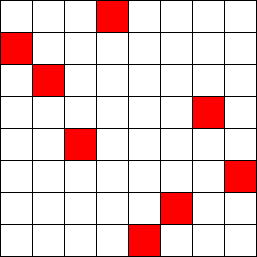
\includegraphics[height=4cm]{Old Scribe Notes/cycle.png}
	\caption{Cycle matrix.}
	\label{fig:cycle}
\end{figure}

\begin{figure}[ht]
	\centering
		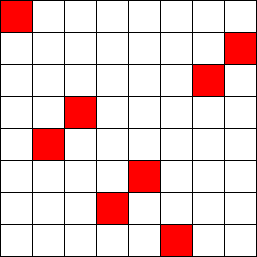
\includegraphics[height=4cm]{Old Scribe Notes/permutation.png}
	\caption{Permutation matrix.}
	\label{fig:permutation}
\end{figure}

Every cycle matrix is a permutation matrix, but the converse is not true.
For each size $n$, there are $n!$ different permutation matrices but
only $(n-1)!$ cycle matrices.

In Figure~\ref{fig:cycle}, one can see the cycle matrix as a cycle $(1,4,7,6,8,5,3,2)$
on the set $\{1,2,3,4,5,6,7,8\}$. In Figure~\ref{fig:permutation}, it is possible to
interpret the matrix as a permutation $(1)(2,8,6,5)(3,7,4)$ on the same set.

\begin{theorem}
There is a non-interactive zero-knowledge (NIZK) proof in the
hidden-bit model (HBM) for the problem of proving that a graph is Hamiltonian.
\end{theorem}
\proof
In the hidden-bit model (HBM), there is a random string $r$ with $\ell$ bits that the prover
can read. The prover should be able to produce a proof $\phi$ and choose a set
$I\subseteq\{1,2,\ldots,\ell\}$ such that the proof and the bits of the string corresponding to
the set $I$ will be revealed to the verifier.
\begin{table}[ht]
\centering
\begin{tabular}{r c l}
%\mright{P}{\phi,I,\{r_i \mid i\in I\}}{V}
\end{tabular}
\end{table}


Let the graph be $G=(V,E)$ with $|V|=n$.
The objective is to convince the verifier that the assertion is correct (the graph $G$
is Hamiltonian).

Suppose that the random string $r$ comes from a distribution
such that this string represents the entries from an $n\times n$ cycle matrix $M_c$.
Then a proof can be produced as follows.

Since the prover $P$ knows the Hamiltonian cycle $x_1,\ldots,x_n$ in $G$, he can find a
function $\phi:V\rightarrow \{1,2,\ldots,n\}$ that puts the Hamiltonian cycle exactly
over the cycle of $M_c$. More precisely, for this function we have
$M_c[\phi(x_i),\phi(x_{i+1})]=1$ for each edge $(x_i,x_{i+1})$ in the Hamiltonian cycle of G
(we view indices modulo $n$).
This means that all the edges of $M_c$ will be covered by edges of $G$. Conversely, all the
non-edges of $G$ must be taken to non-edges of $M_c$.

So the strategy for the prover is to reveal the mapping $\phi$ and also reveal entries of $M_c$ corresponding to $\phi(e)$ where $e \notin E$. More precisely, for the set
$I=\{(\phi(u),\phi(v)) \mid (u,v)\notin E\}$, $P$ reveals
$M_c[\phi(u),\phi(v)]=0$,
which proves that $(\phi(u),\phi(v))$ is a non-edge of $M_c$.

\begin{figure}[ht]
	\centering
		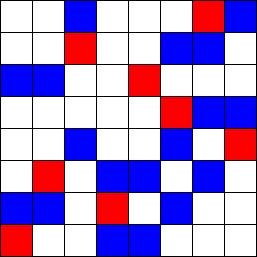
\includegraphics[height=4cm]{Old Scribe Notes/red_blue.png}
	\caption{Graph matrix that includes a Hamiltonian cycle. Edges are blue/red and the
                 cycle is red. White cells are non-edges.}
	\label{fig:red_blue}
\end{figure}

A visual example is shown in Figure~\ref{fig:red_blue}. The cycle graph $M_c$ given by the
random string corresponds to the red cells. These cells have value 1 in the matrix $M_c$ and
all other cells have value 0. The prover $P$ provides a bijection $\phi$ that
maps the edges of $G$ to this matrix in such a way that all red cells are covered and
some others may also be covered (blue cells). The important property guaranteed is that
all the non-edges of $G$ are mapped to cells that have a value 0 in the matrix (white cells).

This proof satisfies the three properties required for a zero knowledge proof.

\textit{Completeness:} if $P$ and $V$ are both honest, then $P$ will be able to convince
$V$ that the statement is true. That's because $P$ knows the Hamiltonian cycle of $G$,
hence he is always able to produce the mapping $\phi$.

\textit{Soundness:} if $P$ is lying and trying to prove a false statement, then he will
get caught with probability 1. If $P$ does not know any Hamiltonian cycle in $G$, then
any function $\phi$ he chooses will not cover all the edges in $M_c$. Hence there will
be an entry in the matrix $M_c$ which is one and will be revealed as a non-edge of $G$.

\textit{Zero Knowledge:} $V$ cannot get any information besides the fact that $P$
knows a Hamiltonian cycle in $G$. A simulator $S$ for this proof can be simply a machine
that generates a random permutation $\phi:V\rightarrow \{1,2,\ldots,n\}$ and reveals zeros
for all the non-edges of $\phi(G)$.

\vspace{5mm}

In this proof we assumed that the random string $r$ comes from a very specific distribution
that corresponds to cycle matrices.
Now we need to show that the general problem (where $r$ comes from a
random uniform distribution of $\ell$ bits) can be reduced into this previous scenario.

We proceed as follows.
Let the length of the random string be
$\ell=\left\lceil 3\cdot \log_2 n\right\rceil \cdot n^4$.
We view the random string $r$ as $n^4$ blocks of $\left\lceil 3\cdot \log_2 n\right\rceil$
bits and we generate a random string $r'$ of length $n^4$ such that each bit in $r'$
is 1 if and only if all the bits in the corresponding block of $r$ are equal to 1.
This way, the probability that the $i$-th bit of $r'$ equals 1 is $\Pr[r'_i=1]\approx\frac{1}{n^3}$ for every $i$.

Then we create an $n^2\times n^2$ matrix $M$ whose entries are given by the bits of $r'$.
Let $x$ be the number of one entries in the matrix $M$.
The expected value for $x$ is $\frac{n^4}{n^3}=n$.
And the probability that $x$ is exactly $n$ is noticeable. To prove that, we can use
Chebyshev's inequality:
$$\Pr[|x-n|\geq n]\leq\frac{\sigma^2}{n^2}=
\frac{n^4\cdot \frac{1}{n^3}\cdot\left(1-\frac{1}{n^3}\right)}{n^2}<\frac{1}{n}.$$
So we have $\Pr[1\leq x\leq 2n-1]>\frac{n-1}{n}$.
And the probability $\Pr[x=k]$ is maximal for $k=n$, so we conclude that
$\Pr[x=n]>\frac{n-1}{n(2n-1)}>\frac{1}{3n}$.

Now suppose that this event ($x=n$) occurred and we have exactly $n$ entries equal to 1
in matrix $M$. What is the probability that those $n$ entries are all in different rows
and are all in different columns?

We can think about the problem this way: after $k$ one entries have been added to the matrix,
the probability that a new entry will be in a different row and different column is given by
$\left(1-\frac{k}{n^2}\right)^2$. Multiplying all these values we get

\begin{align*}
\Pr[\text{no collision}] &\geq \left(1-\frac{1}{n^2}\right)^2 \cdot \left(1-\frac{2}{n^2}\right)^2
\cdots \left(1-\frac{n-1}{n^2}\right)^2 \\
& > 1 - 2\left(\frac{1}{n^2} + \frac{2}{n^2} +\cdots + \frac{n-1}{n^2}\right)
= 1 - \frac{n-1}{n} = \frac{1}{n}.
\end{align*}

Now assume that this event happened: the matrix $M$ has exactly $n$ entries equal to 1
and they are all in different rows and different columns.
Then we can define a new $n\times n$ matrix $M_c$ by selecting only those $n$ rows
and $n$ columns of $M$. By construction, $M_c$ is a permutation matrix.
The probability that $M_c$ is a cycle matrix is $\frac{(n-1)!}{n!}=\frac{1}{n}$.
An example is shown in Figures~\ref{fig:n2}~and~\ref{fig:n}.

\begin{figure}[ht]
	\centering
		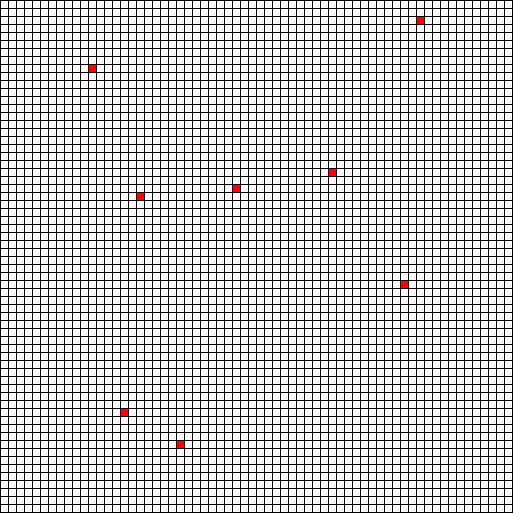
\includegraphics[height=8cm]{Old Scribe Notes/n2.png}
	\caption{Matrix $M$ which is $n^2\times n^2$ for $n=8$.}
	\label{fig:n2}
\end{figure}

\begin{figure}[ht]
	\centering
		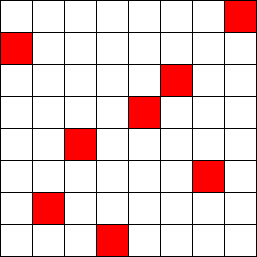
\includegraphics[height=4cm]{Old Scribe Notes/n.png}
	\caption{Matrix $M_c$ which is $n\times n$ for $n=8$. The construction worked,
	         because $M_c$ is a cycle matrix.}
	\label{fig:n}
\end{figure}


Now let's join all those probabilities. The probability that $M_c$ is a cycle matrix is at least
$$\frac{1}{3n}\cdot \frac{1}{n}\cdot \frac{1}{n} > \frac{1}{3n^3}.$$

If we repeat this process $n^4$ times, then the probability that $M_c$ is a cycle matrix in at least one iteration is at least
$$1-\left(1-\frac{1}{3n^3}\right)^{n^4}\approx 1-e^{-\frac{n}{3}} = 1-\mathsf{negl}(n).$$


\bigskip
The proof system works as follows. Given a random string $r$, the prover $P$ tries
to execute the construction above to obtain a cycle matrix.
If the construction fails, the prover simply reveals all the bits in the string $r$
to the verifier, who checks that the constructions indeed fails.
If the construction succeeds, the prover reveals all the entries in the random string $r$
that correspond to values in the matrix $M$ which are not used in matrix $M_c$.
The verifier will check that all these values for matrix $M$ are indeed 0.

Then the prover proceeds as in the previous scenario using matrix $M_c$: he
reveals the transformation $\phi$ and opens all the non-edges.

This process is repeated $n^4$ times. Or, equivalently, a big string of length
$\left\lceil 3\cdot \log_2 n\right\rceil \cdot n^4\cdot n^4$ is used and they are all
executed together. This produces a zero knowledge proof.

\textit{Completeness:} if $P$ knows the Hamiltonian cycle of $G$,
then he will be able to find a suitable transformation $\phi$ whenever a cycle graph is
generated by the construction.

\textit{Soundness:} if $P$ is lying and trying to prove a false statement, then he will
get caught with very high probability. If any of the $n^4$ iterations produces a cycle
graph, then $P$ will be caught. So the probability that he will be caught is
$1-e^{-\frac{n}{3}} = 1-\mathsf{negl}(n)$.

\textit{Zero Knowledge:} again $V$ cannot get any information if the construction succeeds.
And if the construction doesn't succeed, all $V$ gets is the random string $r$, which also
doesn't give any information.
\qed


\begin{theorem}
For any language $L$ in $NP$, there is a non-interactive zero-knowledge (NIZK) proof
in the hidden-bit model (HBM) for the language $L$.
\end{theorem}
\proof
The language $L^*$ of Hamiltonian graphs is $NP$-complete. So any problem in $L$ can
be reduced to a problem in $L^*$. More precisely, there is a polynomial-time function
$f$ such that
$$x\in L \Longleftrightarrow f(x)\in L^*.$$
So given an input $x$, the prover can simply calculate $f(x)$ and
produce a NIZK proof in the hidden-bit model for the fact that $f(x)\in L^*$.
Then the verifier just needs to calculate $f(x)$ and check if the proof for the fact
$f(x)\in L^*$ is correct.
\qed

\begin{theorem}\label{the:NIZK_NP}
For any language $L$ in $NP$, there is a non-interactive zero-knowledge (NIZK) proof
in the common reference string (CRS) model for the language $L$.
\end{theorem}
\proof
In Theorem~\ref{thm:NIZK-amplify} it was shown that any NIZK proof in the hidden-bit model can
be converted into a NIZK proof in the standard (common reference string) model by using
a trapdoor permutation.
\qed
